\scanpage{66}

$X-a$

\diagram{\begin{tikzcd}[column sep=tiny]
\unsure{0|\bullet}\arrow[r]&
H^0_{\unsure{a}}(X,\underline O_X^*)\arrow[r]&
H^0(X,\underline O_X^*)\arrow[r]&
H^0(U,\underline O_X^*)\arrow[r]&
H^{\unsure{1}}_a(X,\underline O_X^*)\arrow[r]&
\underset{\substack{\Vert\\0}}{H^1(X,\underline O_X)}\arrow[r]&
H^1(U,\underline O_X^*)\arrow[r]&
\underline{H^2_a(X,\underline O_X^*)}\arrow[r]&
\underline{H^2(X,\underline O_X^*)}
\end{tikzcd}}

\diagram{\begin{tikzcd}A^*\arrow[r]&\hat A^*\end{tikzcd}}
\margin{$\unsure{m}$}
\[
F\qquad H^0_a(F)
\]

\figure{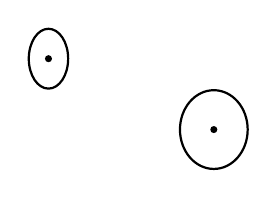
\begin{tikzpicture}[x=1cm,y=1cm]
\draw[thick] (0,1) ellipse (.25 and .38);
\fill (0,1) circle (.045);
\draw[thick] (2.1,.1) ellipse (.43 and .5);
\fill (2.1,.1) circle (.045);
\end{tikzpicture}}

\diagram{\begin{tikzcd}[column sep=large,row sep=large]
\text{loc. factoriel}\arrow[r,Rightarrow]\arrow[dr,Rightarrow]&
\inserted{\text{loc.}}\ \text{quasi-factoriel}\arrow[r,Rightarrow]&
\text{parafactoriel}\\
&\text{\unsure{1} factoriel,}\arrow[d,Rightarrow]&\\
&\text{0-factoriel,}&
\end{tikzcd}}

\diagram{\begin{tikzcd}\widetilde A\arrow[r]&\widetilde A_0\end{tikzcd}}
\deleted{$\unsure{\widetilde A_\xi}$}
\margin{$\longleftarrow$}

\[
H^1(X,\underline O_X)=0
\]

\figure{\begin{tikzpicture}[x=1cm,y=1cm]
\node at (0,.9) {$L$};
\node at (1.1,.9) {$L_B$};
\draw (2.65,1.55) -- (3.7,-.2);
\draw (3.4,1.7) .. controls (3.15,.7) and (2.95,-.35) .. (2.8,-.4);
\fill (3.13,.8) circle (.045);
\node at (5.2,1.8) {$\widetilde X$};
\node at (5.2,.8) {$X$};
\node at (9.7,2.1) {$\Rightarrow$};
\end{tikzpicture}}

\[
J\subset A\subset B
\]
\figure{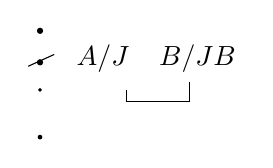
\begin{tikzpicture}[x=1cm,y=1cm]
\fill (-.6,.55) circle (.04);
\fill (-.6,.15) circle (.04);
\draw (-.75,.1) -- (-.42,.25);
\fill (-.6,-.2) circle (.025);
\fill (-.6,-.8) circle (.03);
\node at (.2,.2) {$A/J$};
\node at (1.4,.2) {$B/JB$};
\draw (.5,-.2) -- (.5,-.35) -- (1.3,-.35) -- (1.3,-.1);
\end{tikzpicture}}

\margin{\deleted{$\unsure{1-h=}$}
\[
1-h^1\unsure{=|:}2-h'-h''
\]}

\[
1-g=\sum(1-g_i)-\sum n_s\ \unsure{\ne|=}0
\]
\[
1-g=\nu-\sum g_i-\sum n_s
\]

\figure{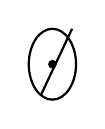
\begin{tikzpicture}[x=1cm,y=1cm]
\draw[thick] (0,0) ellipse (.3 and .45);
\draw[thick] (-.15,-.4) -- (.25,.45);
\fill (0,0) circle (.055);
\end{tikzpicture}}

\margin{\figure{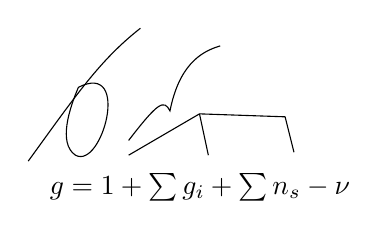
\begin{tikzpicture}[x=.75cm,y=.75cm]
\draw[thin] (0,0) .. controls (.8,1.1) and (1.2,1.7) .. (1.9,2.25);
\draw[thin] (.85,1.25) .. controls (1.75,1.7) and (1.25,-.15) .. (.8,.1)
 .. controls (.5,.3) and (.7,.9) .. (.85,1.25);
\draw (1.7,.1) -- (2.9,.8) -- (4.35,.75) -- (4.5,.15);
\draw (2.9,.8) -- (3.05,.1);
\draw (1.7,.35) .. controls (2.2,1) and (2.3,1.05) .. (2.4,.85)
 .. controls (2.55,1.6) and (2.9,1.85) .. (3.25,1.95);
\node[anchor=west] at (.2,-.45) {$g=1+\sum g_i+\sum n_s-\nu$};
\end{tikzpicture}}}

\[
1-g=1-g'-\sum n_s\qquad
1-g=2-g'-g''-\sum n_s
\]
\[
g=g'+\sum n_s\qquad
g=(g'+g'')+\sum n_s-1
\]

\figure{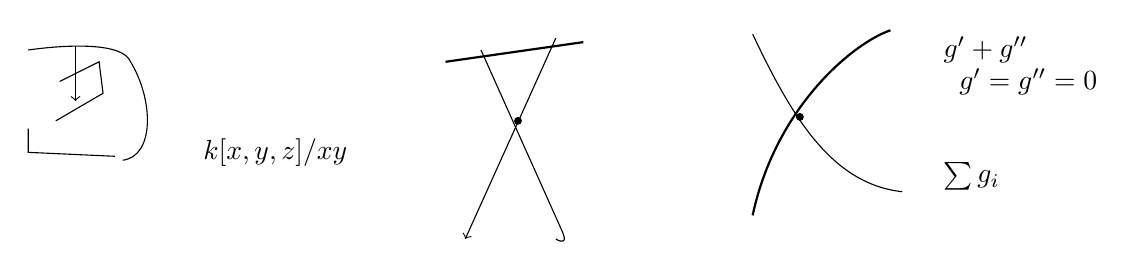
\begin{tikzpicture}[x=1cm,y=1cm]
\draw (-.5,1.05) .. controls (0,1.12) and (.7,1.15) .. (.8,.9)
 .. controls (1.1,.4) and (1.1,-.3) .. (.7,-.35);
\draw (-.5,.05) -- (-.5,-.25) -- (.6,-.3);
\draw (-.15,.15) -- (.45,.5) -- (.4,.9) -- (-.1,.65);
\draw[->] (.1,1.1) -- (.1,.4);
\node[anchor=west] at (1.6,-.25) {$k[\unsure{x},y,z]/xy$};
\begin{scope}[shift={(5.2,.1)}]
\draw[->] (1,1.1) -- (-.15,-1.45);
\draw (.05,.95) -- (1.08,-1.35) .. controls (1.15,-1.5) and (1.08,-1.5) .. (1,-1.45);
\draw[thick] (-.4,.8) -- (1.35,1.05);
\fill (.52,.05) circle (.05);
\end{scope}
\begin{scope}[shift={(8.7,.05)}]
\draw[thick] (0,-1.1) .. controls (.3,.3) and (1.3,1.1) .. (1.75,1.25);
\draw (0,1.2) .. controls (.5,.15) and (1,-.7) .. (1.9,-.8);
\fill (.6,.15) circle (.05);
\node[anchor=west] at (2.3,1) {$\deleted{g'+g''}$};
\node[anchor=west] at (2.5,.6) {$g'=g''=0$};
\node[anchor=west] at (2.3,-.6) {$\sum g_i$};
\end{scope}
\end{tikzpicture}}

\margin{65}
